\begin{frame}[fragile]{MSOX:  A Prototypical Flavoenzyme}
\begin{tikzpicture}[scaleall=1.0]
\pcuad{\textwidth}{\textheight}
%\showcuad
\path (nw) ++(0,0) node (heading) [anchor=north west,text width=\textwidth] 
{MSOX is a bacterial enzyme that uses the \textcolor{orange!80!black}{flavin} redox cycle to catalyze oxidative demethylation of sarcosine to glycine.};
\path(c2) ++(-0.5,0.5) node (FoSr) [shape=rectangle,draw] {F$_{\sf O}$S$_{\sf R}$}
          ++(-2,-1.5) node (Fo) [shape=rectangle,draw] {F$_{\sf O}$}
          ++(+2,-1.5) node (Fr) [shape=rectangle,draw] {F$_{\sf R}$}
          ++(+2,1.5) node (FrPo) [shape=rectangle,draw] {F$_{\sf R}$P$_{\sf O}$}
          ++(-2,-3.5) node (FrPoO2) [shape=rectangle,draw] {F$_{\sf R}$\textcolor{red}{P$_{\sf O}$}O$_{\sf 2}$};
\path(Fo)  +(0.5,1) node (Sr) [shape=rectangle] {S$_{\sf R}$};
\path(FrPo) +(-1.5,0.0) node (Poa) [shape=rectangle] {\textcolor{blue}{P$_{\sf O}$}};
\path(FrPo) +(0.0,-2) node (O2a) [shape=rectangle] {O$_{\sf 2}$};
\path(O2a) +(-2.75,0.0) node (O2b) [shape=rectangle] {O$_{\sf 2}$};
\path(Fo) +(1.5,0) node (H2O2a) [shape=rectangle] {H$_{\sf 2}$O$_{\sf 2}$};
\path(Fo) +(-0.5,-1.5) node (Pob) [shape=rectangle] {\textcolor{red}{P$_{\sf O}$}};
\path(Pob) +(0,-1) node (H2O2b) [shape=rectangle] {H$_{\sf 2}$O$_{\sf 2}$};
\draw [->,thick] (Fo.north east) -- (FoSr.south west) node(attractor1)[pos=0.90]{};
\draw [->,thick,snake] (FoSr.south east) -- (FrPo);
\draw [->,thick] (FrPo.south west) -- (Fr.north east) node(attractor2)[pos=0.10]{};
\draw [->,thick] (Fr.north west) -- (Fo.south east) node (attractor5)[pos=0.10]{} node(attractor4)[pos=0.70]{};
\draw [->,thick] (FrPo.south) -- (FrPoO2.north east) node(attractor3)[pos=0.60]{};
\draw [->,thick] (FrPoO2.north west) -- (Fo.south) node(attractor6)[pos=0.2]{} node(attractor7)[pos=0.6]{};
\draw [<-,thick] (FoSr.south west) .. controls (attractor1.south west) .. (Sr.east);
\draw [->,thick,color=blue] (FrPo.south west) .. controls (attractor2.south west) .. (Poa.south east);
\draw [<-,thick,color=red] (FrPoO2.north east) .. controls (attractor3.south) .. (O2a.west);
\draw [->,thick] (Fr.north west) .. controls (attractor4.north west) .. (H2O2a.south west);
\draw [<-,thick,color=blue] (Fo.south east) .. controls (attractor5.north west) .. (O2b.north);
\draw [->,thick] (FrPoO2.north west) .. controls (attractor6.north west) .. (H2O2b.east);
\draw [->,thick,color=red] (FrPoO2.north west) .. controls (attractor7.north west) .. (Pob.east);
\path(FrPoO2.south) +(0,-0.5) node (sometext) [shape=rectangle,anchor=north] {
\textcolor{blue}{Ping-pong} vs. \textcolor{red}{Modified ping-pong}};
\path(hr) +(0.5,0.0) node (jornsimage) [graphics,anchor=center] {
    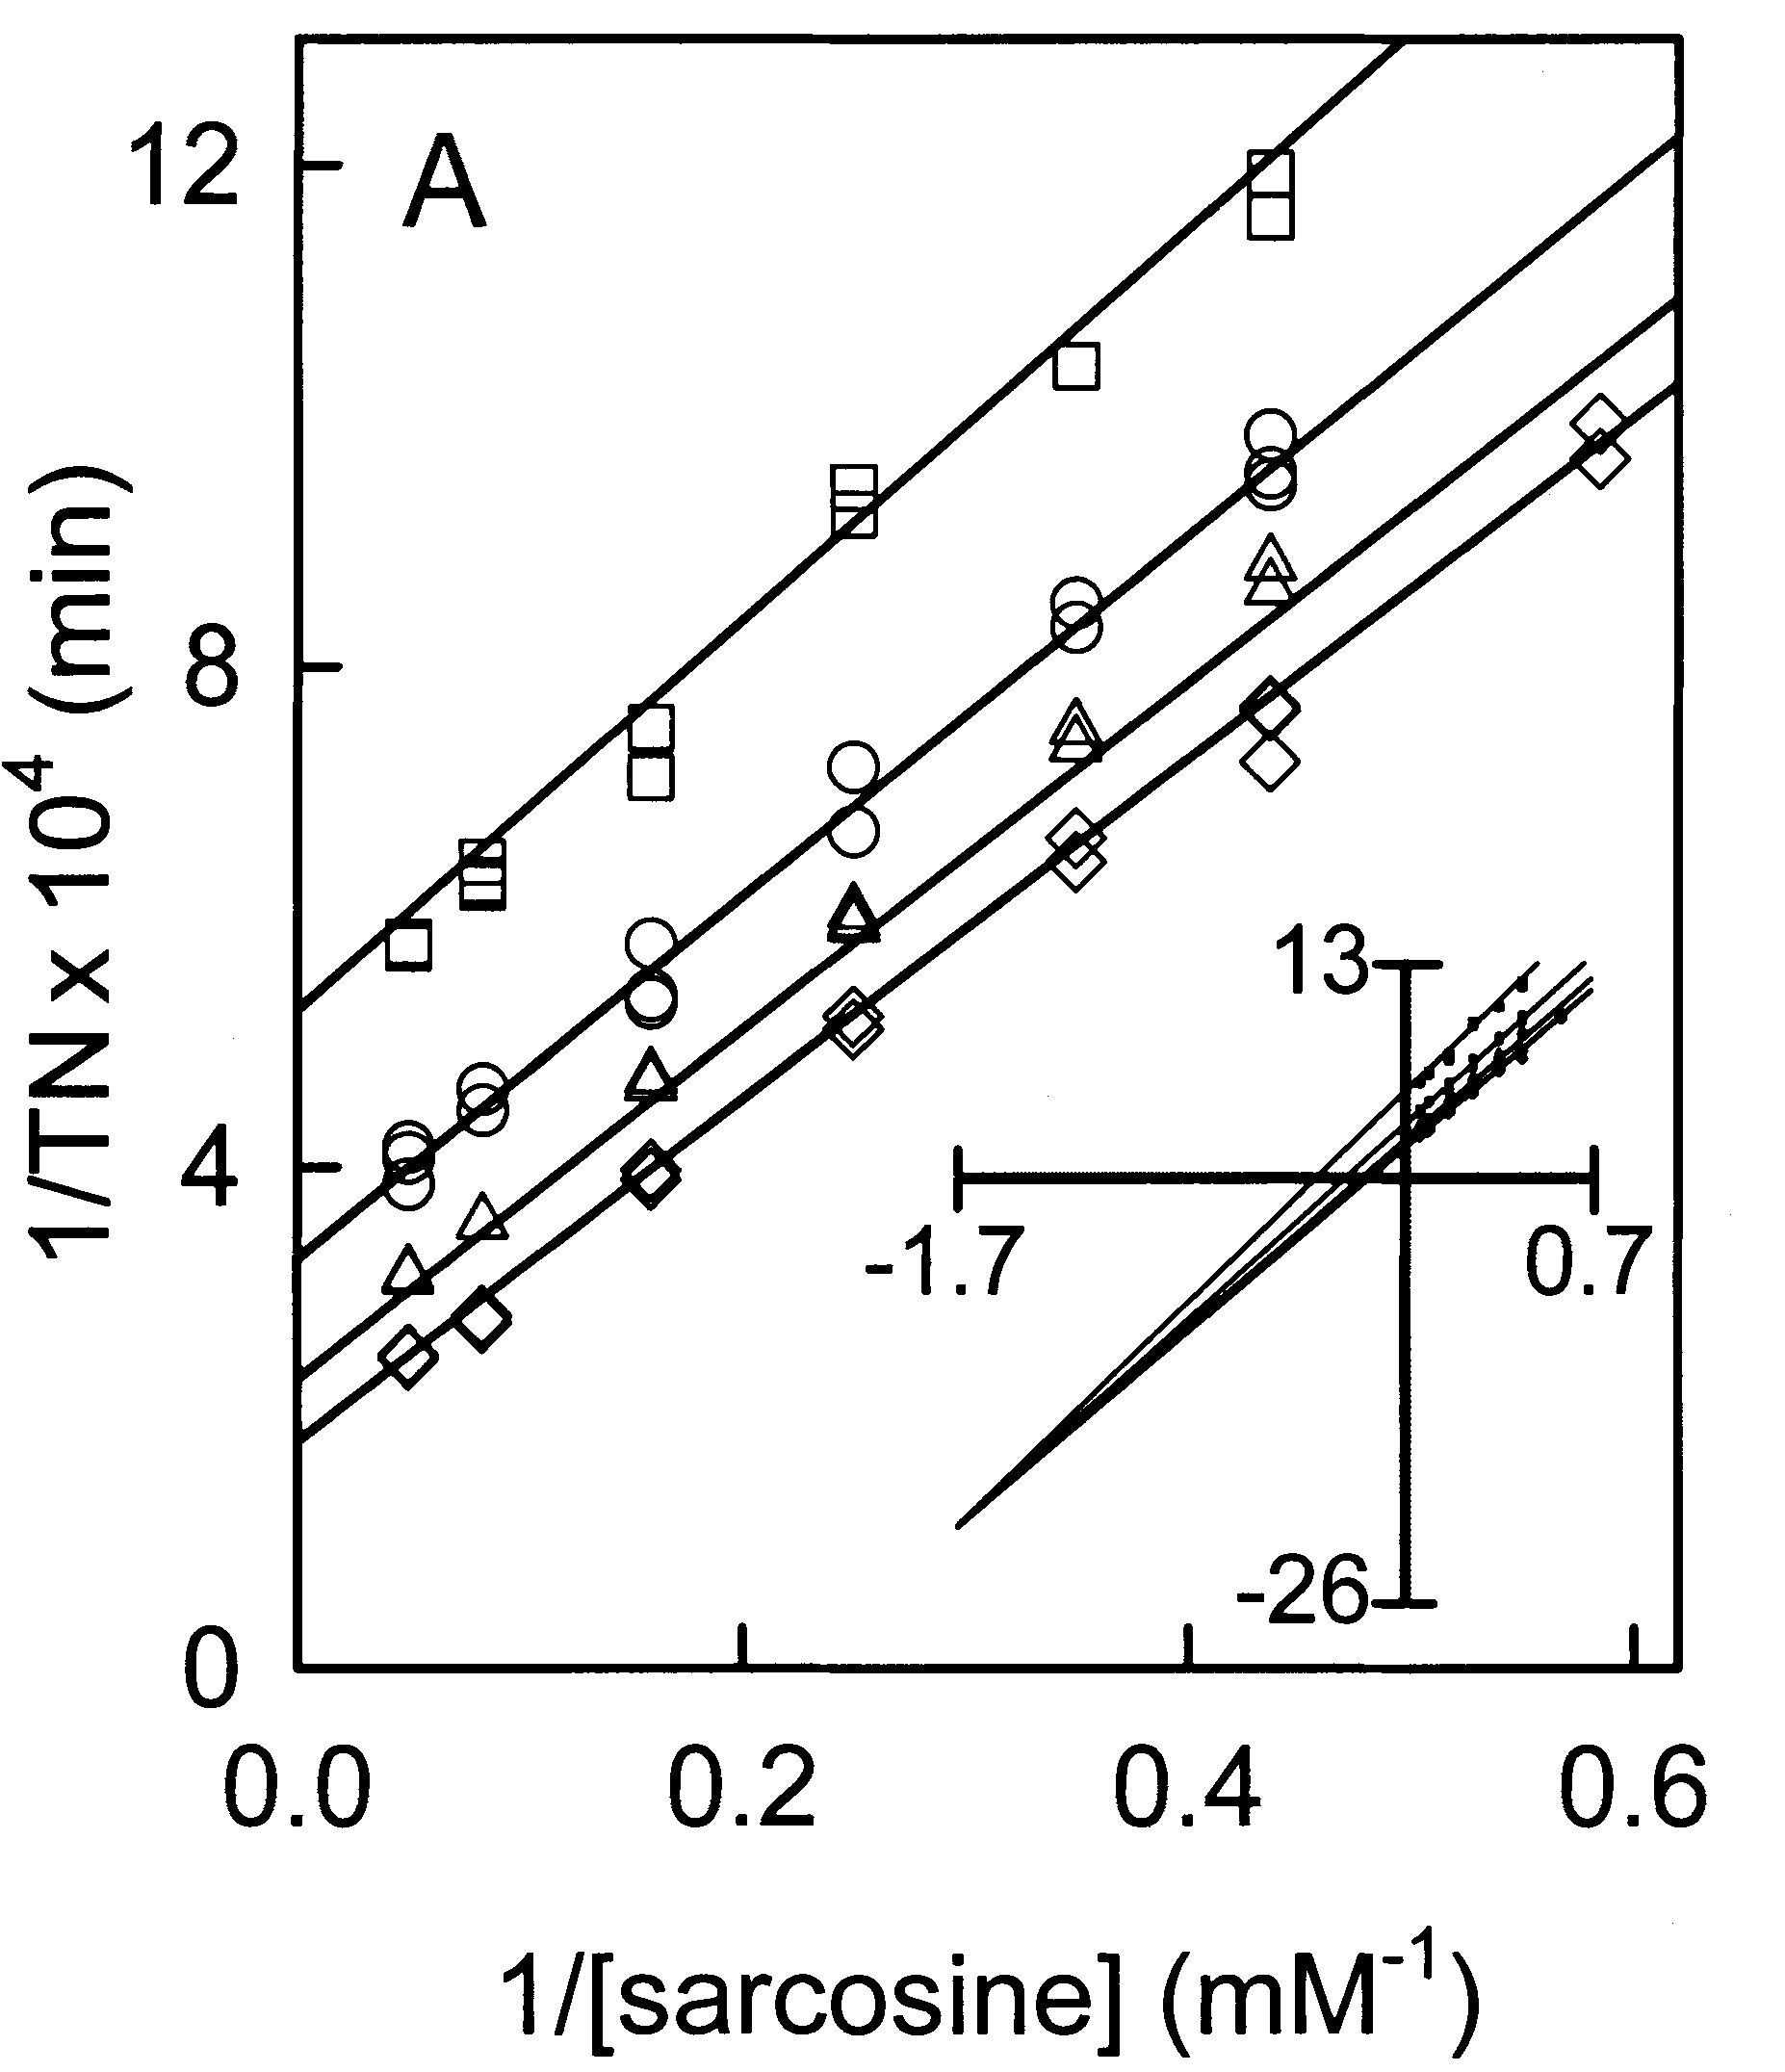
\includegraphics[width=0.5\textwidth]{msox_jorns_expt_2.png}};
\path(jornsimage.south) +(0,-0.2) node(jornsattr)[anchor=center,font=\fontsize{5}{5}\selectfont]{\textcolor{red}{ Zhao, Bruckner, and Jorns, {\it Biochemistry} 2000;{\bf 39}:8825}};
\path(jornsimage.center) ++(-0.5,1.6) node(firstlab)[anchor=center,rotate=39,font=\fontsize{9}{9}\selectfont]{\textcolor{green!80!black}{[O$_2$] = 0.13 mM}}
++(2.15,0.8) node(secondlab)[anchor=center,rotate=39,font=\fontsize{9}{9}\selectfont]{\textcolor{green!80!black}{0.27 mM}}
++(0,-0.5) node(secondlab)[anchor=center,rotate=39,font=\fontsize{9}{9}\selectfont]{\textcolor{green!80!black}{0.56 mM}}
++(0.1,-0.6) node(secondlab)[anchor=center,rotate=39,font=\fontsize{9}{9}\selectfont]{\textcolor{green!80!black}{1.27 mM}};
%0.56, 1.27 
\end{tikzpicture}
\end{frame}
